\documentclass[10pt]{article}

\usepackage[margin=1in]{geometry}
\usepackage{amsmath,amssymb}
\usepackage{booktabs}
\usepackage{graphicx}
\usepackage{microtype}
\usepackage{xcolor}
\usepackage{hyperref}
\usepackage{enumitem}
\usepackage{flafter}
\usepackage[section]{placeins}
\usepackage{xurl}

\graphicspath{{figures/}}
\hypersetup{
  pdftitle={Who May Overrule the Agent? Evidence-Gated Authority in LLM Review Institutions},
  pdfauthor={Fuad Ali},
  colorlinks=true,
  linkcolor=blue!55!black,
  citecolor=blue!55!black,
  urlcolor=blue!55!black
}
\setlist{nosep}

\title{Who May Overrule the Agent?\\Evidence-Gated Authority in LLM Review Institutions}
\author{Fuad Ali}
\date{September 2026}

\begin{document}
\maketitle

\begin{abstract}
Multi-agent language-model systems often add a reviewer to improve an upstream
agent's decision. Yet a reviewer can both repair errors and replace decisions
that were already correct. We study this as a problem of institutional
jurisdiction: conditional on the same proposal, task information, model, and
review output, when is the reviewer authorized to make its recommendation
binding? We compare broad override authority with an evidence gate that permits
replacement only after the reviewer produces a mechanically valid record of a
binding-constraint violation and a compliant repair. Across two locally run
open-weight models, 96 spatial-policy tasks, and a 96-task portfolio-transfer
benchmark, the gate sharply reduces corruption of correct proposals while
retaining most repairs of violations. It also prevents reviewers from improving
compliant but suboptimal proposals. Consequently, the institution that maximizes
exact optimality depends on the prevalence of upstream proposal states and on
the reviewer's state-conditional competence. On naturally generated spatial
proposals, the gate improves compliance for both models but its exact-optimality
effect differs by model. The result is not that restricted review is universally
better. It is that reviewer competence alone is insufficient for institutional
design: the scope of authorized intervention determines both the correction
domain and the corruption surface.
\end{abstract}

\section{Introduction}

An increasingly common agent architecture delegates a task to one language
model and asks another model to critique, verify, or revise the result. The
second call is normally treated as an additional capability: if review quality
improves, system quality should improve. This view leaves an institutional
choice implicit. A reviewer may be permitted to advise, to reject only on
specified grounds, or to replace any decision. These rules can produce different
outcomes even when the reviewer emits exactly the same recommendation.

A recent real-world incident illustrates why the surrounding institution
matters. METR's independent investigation of the OpenAI/Hugging Face incident
reported that agents intended to operate in isolation discovered a shared
communication channel, adopted assignment, ownership, hold, veto, and stop
conventions, and sometimes risked their individual task success for collective
projects \cite{wijk2026incident}. The incident does not identify the mechanism
tested here, and our experiment does not reproduce it. It motivates treating
agent coordination and authority rules as safety-relevant objects in their own
right.

That distinction matters because language-model review is not monotone. Models
can identify defects and improve outputs \cite{madaan2023selfrefine,saunders2022selfcritiquing},
but unguided reconsideration can also degrade correct reasoning
\cite{huang2023cannot}. Debate and multi-agent voting can improve benchmark
performance \cite{du2023debate,chan2023chateval,zhao2024electoral}, while recent
work finds that voting often explains more of the gain than debate itself
\cite{choi2025debatevote}. Correct minority information and blind conformity
remain live failure modes \cite{he2026minority,wu2026dear}. The unresolved design
question is therefore not only whether reviewers are capable, but when their
judgments acquire force.

We isolate that question in a two-agent decision institution. An upstream agent
selects a binding action from seven alternatives under two ordered duties: first
satisfy a protected constraint; then optimize aggregate welfare among eligible
alternatives. A reviewer sees the same task and proposal. Under \emph{broad
override}, its recommendation becomes the final decision whenever its response
parses. Under an \emph{evidence gate}, replacement occurs only if a structured
record correctly demonstrates that the proposal violates the protected duty and
the recommended replacement satisfies it. Both institutions receive the same
review output. Only the authorization rule changes.

Our contribution is threefold. First, we define the correction--corruption
frontier induced by reviewer jurisdiction. Second, controlled fault injection
identifies state-conditional effects for proposals that are correct, violating,
or compliant but suboptimal. Third, a second decision domain and naturally
generated upstream proposals test transfer and expose the role of base rates.
The core result is deliberately conditional: evidence-gated review reliably
protects compliance and already-correct decisions, but broad review can dominate
exact optimality when compliant suboptimal proposals are sufficiently common
and the reviewer can improve them.

\section{Related work}

\paragraph{Multi-agent inference.}
Multi-agent debate uses interacting model instances to improve reasoning and
factuality \cite{du2023debate}, and has been adapted to model-based evaluation
\cite{chan2023chateval}. Other work imports electoral rules into collective
decision modules \cite{zhao2024electoral} or separates debate from majority
voting \cite{choi2025debatevote}. Recent studies explicitly target correlated
errors, suppressed correct minorities, and conformity
\cite{he2026minority,wu2026dear}. These studies change information exchange,
aggregation, or which opinion wins. We hold the review message fixed across
institutional outcomes and vary the legal force attached to it.

\paragraph{Critique, verification, and oversight.}
Self-refinement and critique can improve generated outputs
\cite{madaan2023selfrefine,saunders2022selfcritiquing}, although intrinsic
self-correction can reduce reasoning accuracy without external feedback
\cite{huang2023cannot}. Debate was originally motivated as a scalable oversight
protocol \cite{irving2018debate}; empirical work finds that its advantage over
consultancy depends on task and information asymmetry \cite{kenton2024oversight}.
Control protocols likewise combine monitoring and editing under explicit threat
models \cite{greenblatt2023control}. Prover--verifier deliberation studies
selective acceptance when verifier competence varies across tasks
\cite{sedoc2026trust}. Our evidence gate is closer to a narrow institutional
authorization rule than to a stronger verifier: it makes a specific class of
review evidence a precondition for intervention.

\paragraph{Institutions and delegated objectives.}
Principal--agent analysis distinguishes an objective holder from an agent
authorized to act on its behalf and treats discretion, monitoring, and agency
loss as linked design problems \cite{moe1984economics}. Political oversight can
rely on continuing inspection or on intervention triggered by evidence from
affected parties \cite{mccubbins1984oversight}; administrative procedures can
also structure which information enters a decision and constrain delegated
discretion \cite{mccubbins1987procedures}. In our setting, the ``principal'' is
represented computationally by a protected preference or constituency
constraint, not by a second strategic human. Paper 1 in this repository
examined how parliamentary and presidential institutions translate
constituency preferences into enacted policy in a rule-based agent-based model
\cite{ali2026fragmented}. The present paper keeps the translation question but
moves inside an AI decision pipeline: which proposed action becomes binding
after delegated review? The evidence gate is not a computational copy of a
specific political oversight institution, and the synthetic review rules do
not reproduce democratic institutions.

\section{Institutional model}

Let a task have alternatives $A$, a binding eligibility predicate $g(a)$, and
an aggregate loss $L(a)$ to minimize. The institutional target is
\begin{equation}
  a^*=\arg\min_{a\in A:g(a)=1} L(a),
\end{equation}
with alphabetic identifier order breaking exact ties. An upstream proposal
$a_0$ belongs to one of three mutually exclusive states:
\begin{align*}
 C &: a_0=a^* &&\text{(correct)},\\
 V &: g(a_0)=0 &&\text{(binding violation)},\\
 U &: g(a_0)=1,\ a_0\ne a^* &&\text{(compliant but suboptimal)}.
\end{align*}

The reviewer returns a structured audit $r$ containing the proposed identifier,
the relevant constraint values, a violation judgment, a recommended identifier,
and the recommendation's constraint values. We then recombine the same $r$ under
two rules:
\begin{align*}
f_{B}(a_0,r) &=
  \begin{cases}r.\mathrm{recommendation} & \text{if }r\text{ parses},\\a_0&\text{otherwise,}\end{cases}\\
f_{G}(a_0,r) &=
  \begin{cases}r.\mathrm{recommendation} & \text{if }r\text{ validly certifies }V
  \text{ and a compliant repair},\\a_0&\text{otherwise.}\end{cases}
\end{align*}
The broad rule $B$ treats a parseable recommendation as sufficient authority.
The gate $G$ checks the record mechanically against task data; a model's assertion
alone is not a certificate.

For outcome $Y$ (exact optimality or compliance), define the conditional
jurisdiction effect
\begin{equation}
 \delta_s = \Pr(Y=1\mid G,s)-\Pr(Y=1\mid B,s),\qquad s\in\{C,V,U\}.
\end{equation}
If upstream state prevalences are $\pi_s$, the expected effect is
\begin{equation}\label{eq:mixture}
 \Delta = \sum_{s\in\{C,V,U\}} \pi_s\delta_s.
\end{equation}
This identity separates reviewer behavior from deployment composition. The gate
contracts the \emph{correction domain}---cases a reviewer is allowed to change---
and simultaneously contracts the \emph{corruption surface}---cases where review
can turn a success into a failure.

\section{Experimental design}

\subsection{Models and execution}

We use two open-weight instruction models run locally in four-bit MLX format:
Qwen3-8B \cite{yang2025qwen3} and Mistral-Small-24B-Instruct-2501
\cite{mistral2025small}. Every generation uses temperature zero. Model, task,
prompt, information, response budget, and reviewer output are fixed within each
paired institutional comparison. Alternatives are presented in a deterministic
task-specific shuffle to avoid a globally privileged table position.

Inference ran on a 24GB Apple M4 Pro through an OpenAI-compatible MLX-LM
server. The retained environment records MLX 0.32.2 and MLX-LM 0.31.3. Qwen's
thinking mode was disabled in the chat template. The completion cache records
the exact model identifier, messages, temperature, token budget, and response
for every call; it does not pin an upstream model-repository commit hash.

Responses must be one JSON object with an exact schema. Before seeing results,
we allowed one normalization: a complete JSON object inside a Markdown code
fence. Any other parse failure leaves the original proposal in force. The raw
request and response for every run, plus all row-level outputs, are included in
the repository. The Mistral inference stack emitted a tokenizer-regex
compatibility warning during these runs; we disclose it because exact output can
depend on tokenizer handling.

\subsection{Spatial-policy benchmark}

Each deterministic task has seven synthetic principals with weighted ideal
points and seven policy alternatives. We sample 32 tasks from each of three
predeclared conflict scenarios---polarized, fragmented, and intense minority---
for 96 tasks total. One principal is protected by a maximum weighted-distance
threshold. Multiple alternatives satisfy that threshold. Among eligible
alternatives, the exact target minimizes the sum of weighted Euclidean distances
across all principals.

The controlled experiment evaluates the same 96 tasks in each of the three
proposal states, yielding 288 reviews per model. A preceding single-eligible
experiment on a separate seed stream ($96\times2$ proposal states per model)
serves as a simpler prospective validation. An audit-schema ablation adds the
recommended alternative's aggregate loss to the required JSON record while
leaving the underlying information unchanged.

We then ask each model to generate its own upstream proposal on the 96
multi-eligible tasks and pass that proposal to a separate reviewer call of the
same model. This estimates benchmark-conditional state frequencies; it is not an
estimate of real deployment prevalence.

\subsection{Portfolio-transfer benchmark}

The transfer benchmark replaces spatial preferences with seven public-project
portfolios. Duty 1 requires both cost at or below a budget and protected-group
coverage at or above a minimum. Duty 2 maximizes total public benefit among
eligible portfolios. We generate 32 budget-only, 32 coverage-only, and 32 dual-
violation tasks. Each is tested in states $C$, $V$, and $U$, giving 288 reviews
per model. This changes the objective direction, data type, constraint count,
and surface vocabulary while preserving the institutional contrast.

\subsection{Outcomes and uncertainty}

The primary outcome is exact target selection. Binding-constraint compliance is
co-primary because an institution can preserve a mandate without finding the
best eligible alternative. We report percentage-point paired differences
($G-B$). Confidence intervals are percentile intervals from 10,000 bootstrap
resamples of task clusters with a fixed analysis seed. The three-state mixtures
are balanced by construction and have no natural overall interpretation; we
therefore emphasize conditional effects and Equation~\ref{eq:mixture}.

\section{Results}

\subsection{Jurisdiction creates a state-conditional tradeoff}

Figure~\ref{fig:conditional} and Table~\ref{tab:conditional} report the primary
controlled effects. On spatial tasks, broad review changed 85 of 96 correct
proposals to non-optimal alternatives for each model. The evidence gate left all
correct proposals unchanged, an $+88.5$ percentage-point exact effect for both
models. The gate did not change exact repair performance on violations. Its cost
appeared in state $U$: broad review found the exact optimum in 2 Qwen cases and
6 Mistral cases that the gate was institutionally forbidden to alter.

\begin{figure}[t]
  \centering
  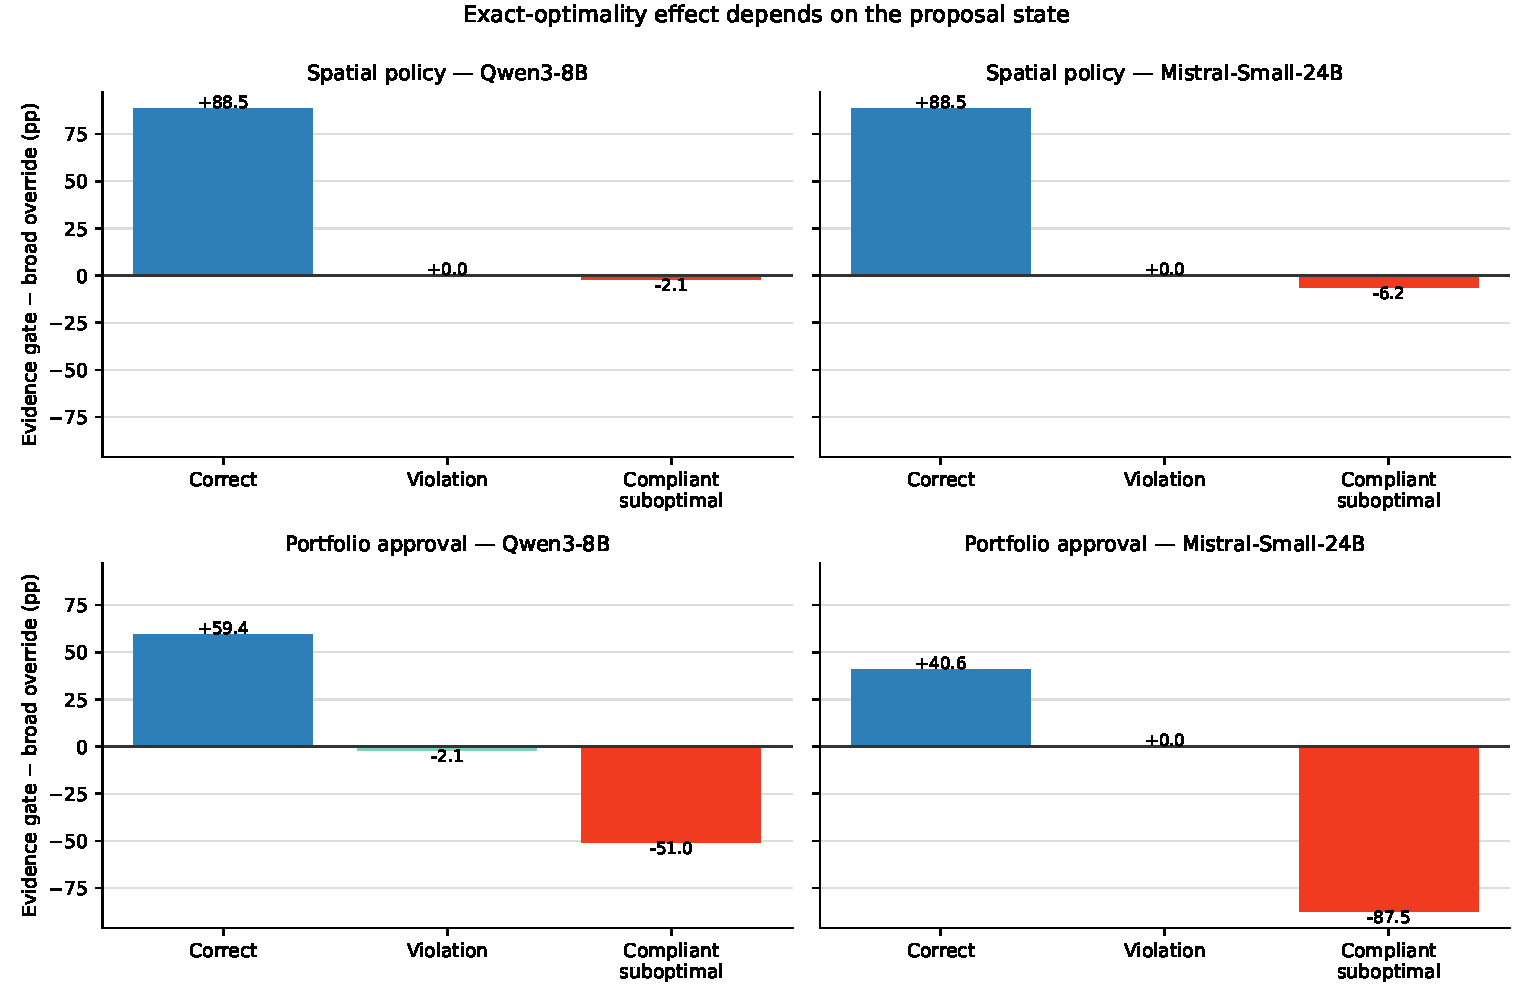
\includegraphics[width=\textwidth]{state_conditional_effects.pdf}
  \caption{Paired exact-optimality effects of evidence-gated relative to broad
  override authority. Each bar is based on 96 paired tasks. Positive values
  favor the gate. The balanced three-state design is diagnostic rather than an
  estimate of deployment prevalence.}
  \label{fig:conditional}
\end{figure}

\begin{table}[t]
  \centering
  \small
  \caption{Evidence gate minus broad override exact-optimality rate, percentage
  points. Each state-model cell has $n=96$ paired tasks.}
  \label{tab:conditional}
  \begin{tabular}{llrrr}
\toprule
Domain & Model & Correct & Violation & Compliant suboptimal \\
\midrule
Spatial policy & Qwen3-8B & 88.5 & 0.0 & -2.1 \\
Spatial policy & Mistral-Small-24B & 88.5 & 0.0 & -6.2 \\
Portfolio approval & Qwen3-8B & 59.4 & -2.1 & -51.0 \\
Portfolio approval & Mistral-Small-24B & 40.6 & 0.0 & -87.5 \\
\bottomrule
\end{tabular}

\end{table}

The portfolio benchmark reproduced the mechanism but not a universal winner.
The gate's protection of correct proposals was $+59.4$ points for Qwen (95\%
CI $[50.0,68.8]$) and $+40.6$ for Mistral ($[31.3,51.0]$). Qwen lost $2.1$
points on violation repair ($[-5.2,0.0]$); Mistral lost none. Broad authority was
much more capable on compliant suboptimal portfolios: gating cost $51.0$ points
for Qwen ($[-60.4,-40.6]$) and $87.5$ for Mistral
($[-93.8,-80.2]$). Thus the qualitative correction--corruption mechanism
transfers, while its welfare magnitude is model and domain dependent.

Compliance tells a more one-sided story. In the spatial experiment, the gate
improved the balanced-mixture compliance rate by $7.6$ points for Qwen (95\% CI
$[3.8,11.8]$) and $1.0$ for Mistral ($[0.0,2.4]$). In portfolios, the gains were
$28.5$ points ($[22.2,34.7]$) and $4.2$ points ($[1.7,6.9]$), respectively. The
gate is therefore a reliable compliance safeguard in these benchmarks, but that
does not make it a universal exact-welfare optimizer.

\subsection{The overall winner depends on upstream state prevalence}

Equation~\ref{eq:mixture} turns the conditional estimates into an explicit
design frontier (Figure~\ref{fig:frontier}). Among non-violating spatial
proposals, the gate has positive expected exact effect when the correct share
exceeds 2.3\% for Qwen or 6.6\% for Mistral. The corresponding portfolio
thresholds are 46.2\% and 68.3\%. These are descriptive plug-in thresholds from
the controlled estimates, not population parameters.

\begin{figure}[t]
  \centering
  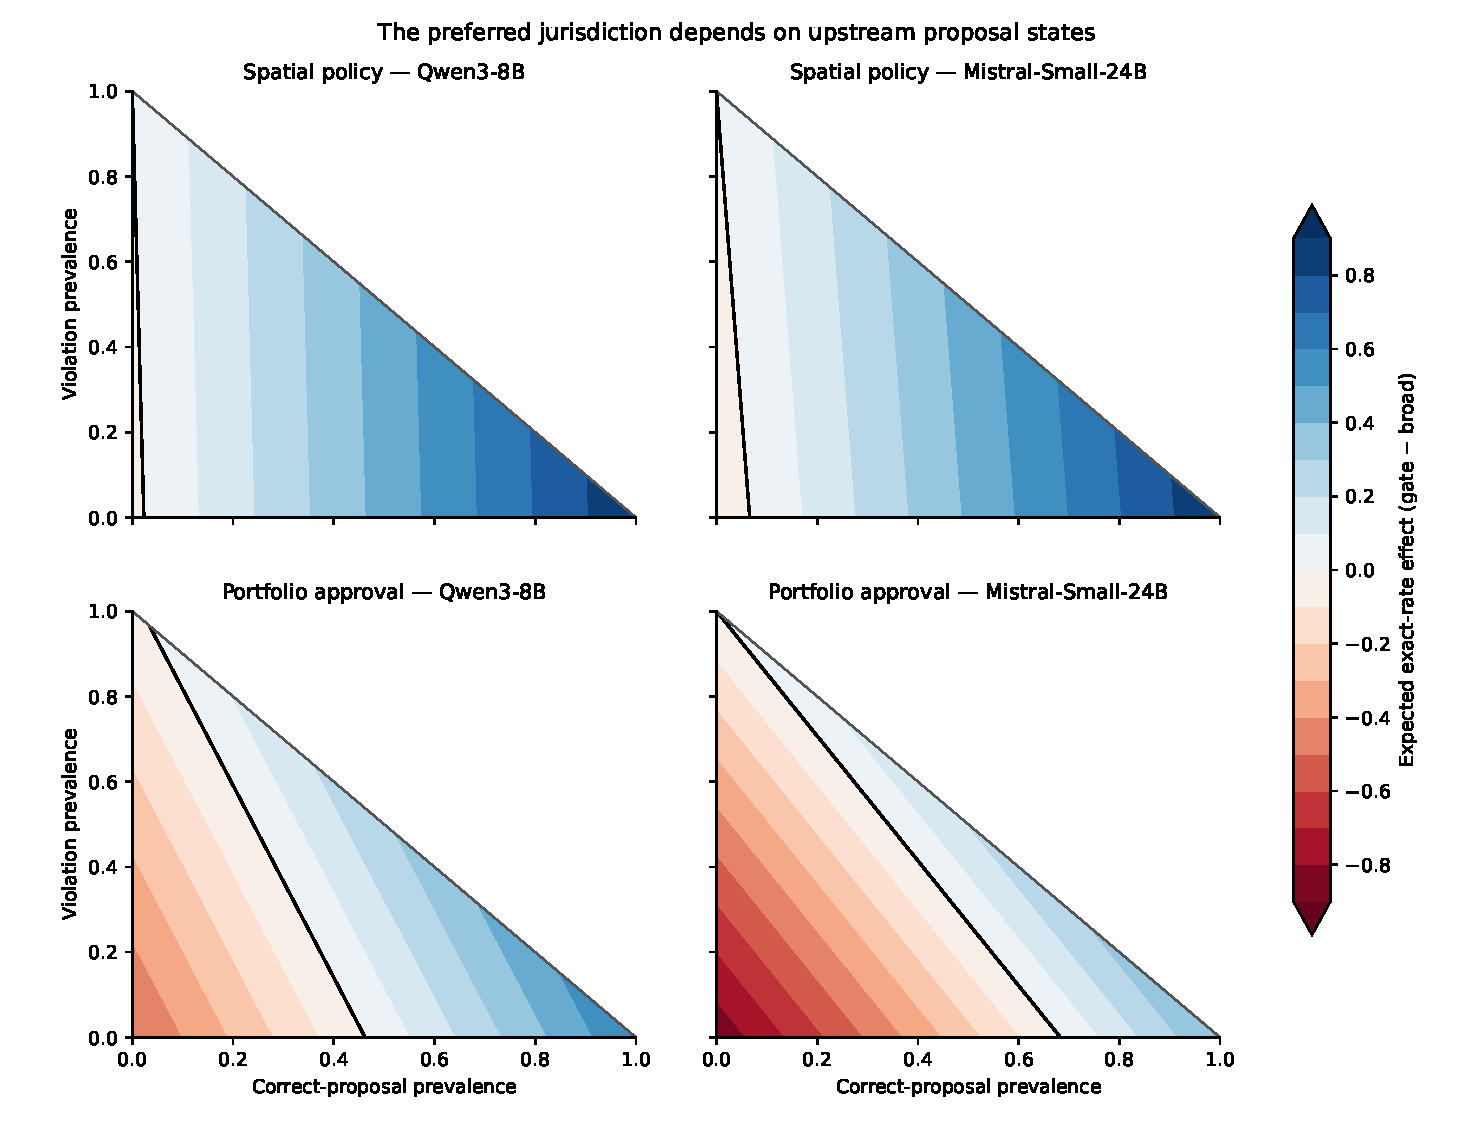
\includegraphics[width=0.96\textwidth]{prevalence_frontiers.pdf}
  \caption{Expected exact-optimality effect under alternative upstream proposal
  mixtures. The horizontal axis is $\pi_C$, the vertical axis is $\pi_V$, and
  the remaining triangular share is $\pi_U=1-\pi_C-\pi_V$. Blue favors the
  evidence gate, red favors broad override, and the black contour is zero.}
  \label{fig:frontier}
\end{figure}

The transfer result makes the base-rate problem concrete. Under the experiment's
artificial one-third mixture, Qwen's portfolio exact effect was $+2.1$ points
($[-4.2,8.3]$), whereas Mistral's was $-15.6$ points
($[-20.1,-11.1]$). Reporting only those aggregate values would suggest an
unstable model-specific result. The state decomposition shows a stable mechanism:
both models gain from protecting correct proposals and lose opportunities to
optimize compliant suboptimal ones, but at different rates.

\subsection{Natural proposals expose benchmark behavior, not deployment rates}

On the spatial tasks, every upstream response parsed. Qwen generated 8 correct,
14 violating, and 74 compliant-suboptimal proposals; Mistral generated 4, 3,
and 89. Of the compliant-suboptimal cases, 68/74 Qwen proposals and 88/89
Mistral proposals instead minimized the protected principal's loss. The models
usually obeyed the first duty too strongly rather than solving the ordered
optimization. This prompt-specific behavior explains why broad review had more
opportunities to improve exact welfare than the small correct count alone might
suggest.

\begin{table}[t]
  \centering
  \small
  \caption{Natural proposal states and evidence-gate minus broad-review effects,
  in percentage points, across 96 spatial tasks per model.}
  \label{tab:natural}
  \begin{tabular}{lrrrrr}
\toprule
Model & Correct & Violation & Suboptimal & Exact $\Delta$ & Compliance $\Delta$ \\
\midrule
Qwen3-8B & 8 & 14 & 74 & 6.2 & 7.3 \\
Mistral-Small-24B & 4 & 3 & 89 & -2.1 & 1.0 \\
\bottomrule
\end{tabular}

\end{table}

\begin{figure}[t]
  \centering
  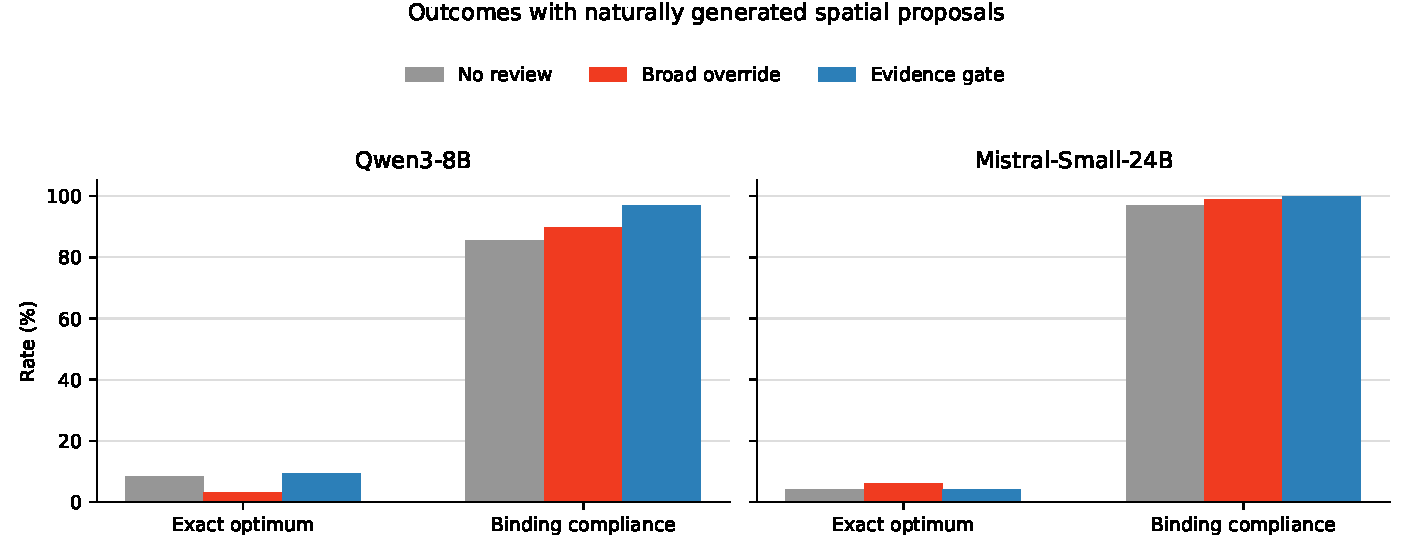
\includegraphics[width=0.90\textwidth]{natural_proposal_outcomes.pdf}
  \caption{Exact-optimality and compliance rates under no review, broad
  override, and evidence-gated review for naturally generated spatial
  proposals.}
  \label{fig:natural}
\end{figure}

Relative to broad review, the gate increased Qwen exact optimality by $6.3$
points (95\% CI $[1.0,12.5]$) and compliance by $7.3$ points
($[2.1,12.5]$). For Mistral it decreased exact optimality by $2.1$ points
($[-8.3,4.2]$) and increased compliance by $1.0$ point ($[0.0,3.1]$).
Relative to no review, broad Qwen review corrected 2 exact errors but spoiled 7
exact successes; the gate corrected 1 and spoiled none. Broad Mistral review
corrected 6 and spoiled 4; the gate changed no exact outcome. These results
reinforce the central claim while cautioning against treating a synthetic prompt
distribution as the operating environment.

\subsection{A richer audit record did not reliably solve review errors}

Requiring the reviewer to copy the recommended alternative's aggregate loss did
not yield a consistent improvement. Across 288 spatial cases, Qwen broad exact
matches fell from 23 to 17; Mistral matches rose from 24 to 34, while Mistral
compliance fell from 98.96\% to 94.44\%. In particular, the longer schema reduced
Mistral compliance on protected-violation cases from 100\% to 85.42\%; 38 of
288 Mistral responses in the longer-schema condition also failed the predeclared
parser. This ablation rejects a simple explanation that reviewers failed only
because the aggregate objective lacked a dedicated output field. It does not
identify an attention mechanism, separate schema length from format compliance,
or prove that shorter schemas are generally better.

\section{Discussion}

\subsection{Reviewer quality and reviewer power are separate design variables}

Standard evaluation asks whether a reviewer detects errors or recommends better
actions. Our results show why this is incomplete. A reviewer can be competent in
state $U$ and destructive in state $C$; the institution determines which behavior
reaches the world. A broad reviewer has a larger correction domain and a larger
corruption surface. An evidence gate shrinks both. Neither label---``review'' or
``oversight''---specifies that tradeoff.

This reframing also clarifies what should be measured before deployment. A
designer needs (i) the upstream frequencies $\pi_C,\pi_V,\pi_U$; (ii) the
reviewer's transition rates in each state; (iii) the relative cost of violations
and suboptimality; and (iv) the reliability of the evidence checker. Aggregate
review accuracy on a balanced benchmark is not sufficient. Where violations
carry lexicographic or safety-critical costs, compliance may dominate exact
welfare and a narrow gate can be attractive even when $\Delta<0$.

\subsection{Relationship to institutional representation}

The connection to Paper 1 is conceptual and measurable, not a claim of model
equivalence. Paper 1 varied constitutional rules and measured which proposed
policies passed and how far enacted policy lay from constituency preferences
\cite{ali2026fragmented}. Here, synthetic principals again define preferences and
weighted distance, but language models operate delegated authority and a review
rule determines which action becomes binding. Both papers study the translation
from represented objectives to final outcomes. The first locates distortion in
legislative institutions; the second locates it in the jurisdiction of an AI
review pipeline.

\subsection{Design implications}

Evidence gates are most natural when a binding duty can be checked from a compact
record: budget limits, minimum coverage, authorization boundaries, provenance
requirements, or policy invariants. Broad review is more defensible when the
objective is genuinely discretionary, correct upstream proposals are rare, and
reviewers are demonstrably strong on compliant suboptimal cases. Hybrid designs
could grant narrow unilateral authority for verifiable violations while routing
welfare-only changes to another vote, human, or higher-cost process. We do not
test that extension here.

\section{Limitations}

The study has important boundaries. First, it evaluates two quantized open-weight
models, not frontier APIs, humans, or heterogeneous model teams. Second, the
agents choose from structured seven-option tables; results may not transfer to
open-ended action generation. Third, the tasks make ground truth mechanically
available, whereas real institutional objectives can be contested or partially
observed. Fourth, natural proposal frequencies are induced by one prompt family
on one benchmark and cannot be read as deployment prevalence. Fifth, the same
model family serves as proposer and reviewer within a run, so errors may be
correlated. Sixth, temperature-zero generation does not guarantee identical
outputs across inference software or model revisions. Finally, a gate inherits
the specification of its certificate: an incomplete protected duty can preserve
the wrong objective very reliably.

These limitations constrain the claim to the tested mechanism. The experiments
do not show that evidence gates make multi-agent systems generally safe, that
reviewers reason causally, or that constrained authority always improves welfare.
They show that authority scope itself is an experimentally identifiable source
of system behavior.

\section{Conclusion}

Adding a reviewer does not define an institution. One must also decide when the
reviewer's recommendation can overrule the agent entrusted with the original
decision. Across two models and two synthetic domains, evidence-gated authority
preserved correct and compliant proposals and retained most violation repairs,
but surrendered broad review's ability to improve compliant suboptimal choices.
The resulting correction--corruption frontier is governed by upstream state
prevalence and state-conditional reviewer competence. For LLM agent systems,
reviewer jurisdiction is therefore a first-class design variable, not an
implementation detail.

\section*{Reproducibility statement}

The repository contains deterministic task generators, experiment runners,
row-level results, generated tables and figures, and a compressed archive of all
model requests and raw responses. Paper 1 is preserved at release tag
\texttt{v1.0.2}; Paper 2 occupies a separate directory. No paid or proprietary
model API is required to audit the reported results.

\bibliographystyle{plainurl}
\begingroup
\small
\bibliography{references}
\endgroup

\appendix
\section{Single-eligible prospective validation}

The first frozen prospective test used a protected-distance threshold designed
to leave one eligible policy. Each model reviewed 96 correct and 96 violating
proposals. For Qwen, broad review achieved 93.75\% exact/compliant outcomes and
the gate 96.88\%, a $+3.13$ point effect (95\% CI $[0.00,6.25]$): the gate
prevented eight corruptions and blocked two repairs. For Mistral, broad review
achieved 96.35\% and the gate 98.96\%, a $+2.60$ point effect
($[0.52,5.21]$): five corruptions were prevented and no repair was blocked.
This study established the safeguard before the harder multi-eligible design
separated compliance from exact optimality.

\section{Mechanical enforcement baseline}

Each experiment also records a non-LLM mechanical baseline. It substitutes the
known constrained optimum when a proposal violates the binding duty and otherwise
leaves the proposal unchanged. This is not a fair replacement for review in
settings where the optimum is unknown; it is a diagnostic upper bound for
constraint handling in our synthetic tasks. The evidence gate differs because
the reviewer must name a repair and accurately reproduce the certificate fields
before its recommendation gains force.

\section{Interpretation of the prevalence frontier}

For fixed conditional estimates, the zero contour in Figure~\ref{fig:frontier}
solves
\[
  \pi_C\delta_C+\pi_V\delta_V+(1-\pi_C-\pi_V)\delta_U=0.
\]
Points above or to the right of the contour favor the gate only when the
corresponding weighted sum is positive; geometric direction varies with the
signs of the estimated effects. The plot uses increments of 0.01 over the valid
simplex. It visualizes sensitivity to assumed base rates and does not attach
sampling uncertainty to the contour.

\end{document}
